\documentclass[runningheads]{llncs}

\usepackage[utf8]{inputenc}
\usepackage[numbers, comma, sort]{natbib}
\bibliographystyle{apalike}

\usepackage{amssymb}
\setcounter{tocdepth}{3}
\usepackage{graphicx}
\usepackage{float}

\usepackage{wrapfig}


\usepackage{pgfplots}
\usepackage{tikz}
\usetikzlibrary{arrows,backgrounds,positioning}


\usepackage{url}
\urldef{\mailsa}\path|rob@clabs.cc,schubotz@tu-berlin.de |
\newcommand{\todaydate}{\leadingzero{\day}.\leadingzero{\month}.\the\year}
\newcommand{\keywords}[1]{\par\addvspace\baselineskip
\noindent\keywordname\enspace\ignorespaces#1}

\begin{document}

\mainmatter

\title{Mathematical Language Processing \\ Project}
\titlerunning{MLP}

\author{Robert Pagel \and Moritz Schubotz}
\authorrunning{Pagel, Schubotz}

\institute{
Database Systems and Information Management Group,\\
Technische Universit\"{a}t Berlin,
Einsteinufer 17, 10587 Berlin, Germany\\
\mailsa\\
\url{http://demo.formulasearchengine.com/}}


\maketitle


\begin{abstract}
In natural language, words and phrases themselves imply the semantics.
In contrast, the meaning of identifiers in mathematical formulae is undefined.
Thus scientists must study the context to decode the meaning.
The \emph{Mathematical Language Processing} project aims to support that process and
presents automated identifier definition discovery.
Ordinary natural language processing approaches are trained on large, manually annotated news
corpora for instance.
They fall short in reasonable quality of definition discovery for scientific texts.
We use statistical methods to discover definitions in the surrounding text.
The evaluation of our prototypical system, applied on the Wikipedia text
corpus, shows that our approach augments the user experience
substantially.
While hovering the identifiers in the formula, tool-tips with the most probable definitions
occur.
Tests with random samples show that the displayed definitions provide
a good match with the actual meaning of the identifiers.   
\keywords{definition discovery, text mining, parallel computing}
\end{abstract}


\section{Introduction}

Mathematical formulae are a viable source of information for a wide range of
scientists.
Often, they contain variables that are unknown or ambiguous to the reader.
Therefore, one usually needs to study the surrounding text to find the relevant definition.
An automatic information retrieval system can be used to reduce the reader's
effort.
Students and scientists of other disciplines would especially profit from a 
system that helps them to understand formulae.

To build such a system, a labeled text corpus that annotates variables
and their definition is desirable.
At the project start, such a corpus was not available.
We use simple statistical assumptions about co-occurrences between identifiers
and their potential definition to extract the meaning of the identifiers from their context.
In combination with the Stratosphere system
that is capable of scalable data processing,  we rapidly generate a large amount of 
definition relation 
candidates with only minimal implementation overhead to ensure the scalability of our algorithm.

%\pagebreak
\begin{wrapfigure}{r}{0.5\textwidth}
        \label{fig:screenshot}
  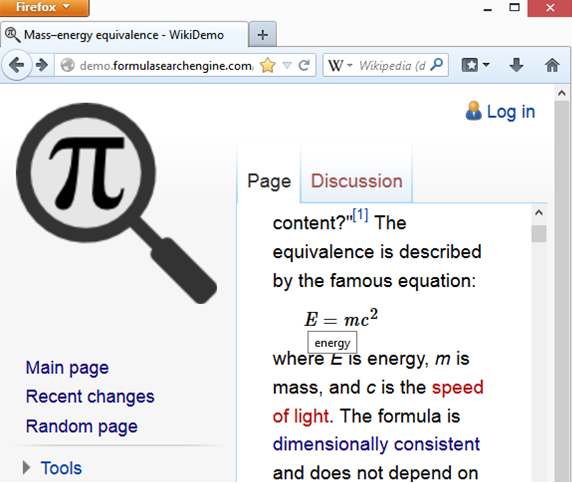
\includegraphics[width=0.5\textwidth]{screenshot}
  \caption{Screenshot of the energy mass relation page `Mass–energy equivalence', while hovering the letter `E'.}
  \vspace{-20pt}
\end{wrapfigure}
We chose the Wikipedia text corpus as a target because of two facts.
First, because the input language for formula texvc is very restrictive, it is easy to extract the formulas and identifiers from the text.
Second, we are able to leverage the semantic information between mark-up and
word tokens, e.g., hyperlinks.

The English Wikipedia contains roughly four million articles.
Even if we only
pick articles containing the \texttt{<math/>} tag, our processor still needs
to compute with tens of thousands of articles.
Especially when using a maximum
entropy \emph{POS} tagger \cite{Rathna96}, like the one in Stanford's NLP
framework, one can make use of a parallel processing system to speed up
computation.
Therefore we implement the proposed strategy with the Stratosphere system based
on the PACT programming model \cite{Alexandrov2010}.


\paragraph{Related Work.}

\citeauthor{Quoc2010} \cite{Quoc2010} proposed an approach for
relating whole formulas to sentences and their describing paragraphs.
\citeauthor{Yokoi} \cite{Yokoi} trained a \emph{support vector machine} to extract
natural language descriptions for mathematical expressions.


\section{Statistical definition discovery}

We detect relations between identifiers and their description in two steps.
First, we extract the identifiers from the formulae and
second we determine their description from the surrounding text.

Inspired by the \emph{Distant Supervision} approach \cite{Mintz2008},
we assume that the identifier and the definition co-occur in the same sentence.
Each description candidate is scored with the weighted sum
\begin{equation} \label{eq:rating}
R(n,\Delta,t,d)=\frac{\alpha{R}_{\sigma_\mathrm d}(\Delta)
+\beta{R}_{\sigma_\mathrm s}(n)
+\gamma\mathrm{tf}(t,d)}{\alpha+\beta+\gamma} \mapsto [0;1].
\end{equation}
It depends on the distance $\Delta$ between identifier and definition term $t$, the distance $n$ between the display-style equation and the sentence that contains the term, and the identifier and the term frequency $\mathrm{tf}(t,d)$ in the current document $d$.
The distance was normalized with $R_\sigma(\Delta)= \exp\left[-\frac{1}{2}\frac{\Delta^2-1}{\sigma^2}\right].$
We assume that the probability to find a relation at $\Delta=1$ is maximal.  For example in the 
text fragment \emph{the energy $E$, and the mass $m$,}  
in order to determine the full width at half maximum of our distribution, we evaluated some articles manually and found $R_{\sigma_\mathrm d}(1)\approx 2 R_{\sigma_\mathrm d}(5)$ and thus 
$\sigma_d=\sqrt\frac{12}{\ln 2}$.
The probability to find a correct definition decays for 50\% within three sentences.
Consequently  $\sigma_\mathrm s=2\left({\ln 2}\right)^{-\frac{1}{2}}$.

The classic tf-idf \cite{Salton86} statistic reflects the importance of a term to a document.
For our task, the inverse document frequency (idf) would assign high penalties to 
frequent words like `energy', in comparison to 
%\todo{I replaced `seldom words' with `words seldom seen'.  Is that ok?}
words seldom seen like `Einstein', which are valid definitions for identifiers.
As the influence of $\mathrm{tf}(t,d)$ on the overall ranking (\ref{eq:rating}) seems to be very high, we reduce the impact with the tuning parameters $\gamma=0.75$ and $\alpha = \beta = 1$.

\paragraph{Implementation.}
We implemented the MLP processing system \cite{github} as Stratosphere data-flow using Java which allows for scalable execution, application of complex higher order functions and easy integration of third party tools like Stanford NLP and the Mylyn framework.
\section{Evaluation}
We extracted 460 identifiers definition tuples in 550000 relations with a
high score ($>0.8$).  The most common identifier definition tuples were 
number $n$ (1709), time $t$ (1480), mass $M$ (1042), radius $r$ (752), 
temperature $T$ (666), angle $\theta$ (639), group $G$ (635).
Because we do not have any annotated test corpora,
evaluation has to be performed by hand.
Therefore, we took a sample of 30
random documents and counted all matches.
Most of the retrieved definitions were considered as relevant.
Furthermore, for more than 50\% of the investigated identifiers, 
the most probable meanings detected by our system were relevant.
However, we neither consider identifiers with subscripts, nor identifiers that do not occur in the surrounding text.  
%The resulting estimates for
%\emph{recall} and \emph{precision} are 0.99 and 0.86 respectively.



\section{Further work}
Our original intuition was to discover grammatical patterns 
like \emph{let \texttt{variable} be \texttt{definition}} or 
were \emph{\texttt{variable} (indicates/stands for/denotes) \texttt{definition}} based on the statistical findings.
However, our impression is that this 
would not lead to significant performance gain.

The distance measure
$R_{\sigma_d}$
fails for the example of Fig.~\ref{fig:screenshot} since
$\Delta(\mathsf{energy},E)=\Delta(\mathsf{mass},m)=2$.
We plan to consider the grammatical structure of the sentence for an improved distance measure $\Delta^{+} : \Delta^+(\mathsf{energy},E)\ge\Delta^+(\mathsf{mass},m)$.
Currently, we use the score $R$ to identify the most probably definition-identifier tuple on each page, even if it occurs multiple times on the page.
For example, on the `Mass-energy equivalence' page, 21 sentences contain the combination of the identifier $E$ and the noun `energy'.
A promising approach, is to use $R^\Sigma=\sum_{i=1}^n 2^{-i} R_i,$ where $R_i$ is a 
sorted list, were $R_1$ is the highest ranked definition for that relation according to the current measure $R$.
To improve the robustness of the \emph{term frequency} measure further, one
might cluster sets of scientific documents, based on their specific fields of
research.


\section{Conclusion}
Our experiments showed that combining a POS tagger with numerical statistics
about the text surface, can lead to quality results.
However, this approach is
only applicable under certain conditions. 
For identifiers which
are seldom seen, our statistical approach tends to fail.
In that situation, other methods, especially supervised ones, are used to
bootstrap a language model.
Unfortunately, they require a labeled test
corpus to measure the performance of a classifier that could be trained with our generated data.
Currently, we are planning to use the
NTCIR-Math-10 Task, Math Understanding Subtask gold standard dataset \cite{overview}
for a comparable evaluation.
Furthermore, a systematic approach for determining a wise choice of the ranking parameters should significantly improve the overall performance of our system.
\paragraph*{Acknowledgments.}
Thanks to Howard Cohl for proof reading the paper and to Holmer Hemsen, the course instructor of the database project course at TU-Berlin in Fall 2012. The implementation and a first draft of this paper was completed in the duration of this course.


\begingroup
\let\clearpage\relax
\bibliography{mlp-papers}
\endgroup

\end{document}

